\documentclass[a4paper]{MBE}
\usepackage[bookmarks]{hyperref}
\hypersetup{
	colorlinks,
	citecolor=black,
	filecolor=black,
	linkcolor=black,
	urlcolor=black
}
\usepackage{amssymb,amsfonts,amsmath,amsthm,mathtools}
\usepackage{lmodern}
\usepackage{bm,bbold}
\usepackage{xfrac, nicefrac}
\usepackage{graphicx}
\graphicspath{{artworks/}}
\usepackage{tikz}
\usetikzlibrary{positioning}
\usetikzlibrary{arrows,automata}
\pdfinclusioncopyfonts=1

\definecolor{RED}{HTML}{EB6231}
\definecolor{YELLOW}{HTML}{E29D26}
\definecolor{BLUE}{HTML}{5D80B4}
\definecolor{LIGHTGREEN}{HTML}{6ABD9B}
\definecolor{GREEN}{HTML}{8FB03E}
\definecolor{PURPLE}{HTML}{BE1E2D}
\definecolor{BROWN}{HTML}{A97C50}
\definecolor{PINK}{HTML}{DA1C5C}

\newcommand{\der}{\mathrm{d}}
\newcommand{\e}{\mathrm{e}}
\newcommand{\dnds}{dNdS}
\newcommand{\indice}{l}
\newcommand{\indiceexp}{^{(\indice)}}
% Time, effective population size and mutation rate.
\newcommand{\Ne}{N}
% \acrshort{DNA}
\newcommand{\SetNuc}{\Omega_{\mathrm{N}}}
\newcommand{\SetWeak}{\Omega_{\mathrm{W}}}
\newcommand{\SetStrong}{\Omega_{\mathrm{S}}}
\newcommand{\mutmatrix}{R}
\newcommand{\Mutmatrix}{\bm{\mutmatrix}_{4\times4}}
\newcommand{\exchan}{\rho}
\newcommand{\Exchan}{\bm{\exchan}_{6\times1}}
\newcommand{\mutequi}{\sigma}
\newcommand{\Mutequi}{\bm{\mutequi}_{4\times1}}
% Codons
\newcommand{\SetCodon}{\Omega_{\mathrm{C}}}
\newcommand{\ci}{{i}}
\newcommand{\cj}{{j}}
\newcommand{\itoj}{\ci, \cj}
\newcommand{\nucitoj}{\mathcal{M}(\itoj)}
\newcommand{\submatrix}{Q}
\newcommand{\Submatrix}{\bm{\submatrix}_{61\times61}}
\newcommand{\subequi}{\pi}
\newcommand{\Subequi}{\bm{\subequi}_{61\times1}}
\newcommand{\probmatrix}{P}
\newcommand{\Probmatrix}{\bm{\probmatrix}_{61\times61}}
% Amino-acids
\newcommand{\SetAa}{\Omega_{\mathrm{A}}}
\newcommand{\Neighbor}{\mathcal{V}}
\newcommand{\NonSyn}{\mathcal{N}}
\newcommand{\Syn}{\mathcal{S}}
\newcommand{\Nx}{\Neighbor_x}
\newcommand{\NxAB}{\Neighbor_x^{\mathrm{A} \rightarrow \mathrm{B}}}
\newcommand{\NyBA}{\Neighbor_x^{\mathrm{B} \rightarrow \mathrm{A}}}
\newcommand{\NxWS}{\Neighbor_x^{\mathrm{W} \rightarrow \mathrm{S}}}
\newcommand{\NxSS}{\Neighbor_x^{\mathrm{S} \rightarrow \mathrm{S}}}
\newcommand{\NxSW}{\Neighbor_x^{\mathrm{S} \rightarrow \mathrm{W}}}
\newcommand{\NxWW}{\Neighbor_x^{\mathrm{W} \rightarrow \mathrm{W}}}
\newcommand{\NyWS}{\Neighbor_y^{\mathrm{W} \rightarrow \mathrm{S}}}
\newcommand{\NySS}{\Neighbor_y^{\mathrm{S} \rightarrow \mathrm{S}}}
\newcommand{\NySW}{\Neighbor_y^{\mathrm{S} \rightarrow \mathrm{W}}}
\newcommand{\NyWW}{\Neighbor_y^{\mathrm{W} \rightarrow \mathrm{W}}}
\newcommand{\NxNonSyn}{\NonSyn_x}
\newcommand{\NyNonSyn}{\NonSyn_y}
\newcommand{\NxSyn}{\Syn_x}
\newcommand{\NySyn}{\Syn_y}
\newcommand{\aminoacid}{\text{A}}
\newcommand{\aai}{\mathcal{A}(\ci)}
\newcommand{\aaj}{\mathcal{A}(\cj)}
\newcommand{\Ni}{\mathcal{N}_{\mathrm{eighbors}}\left(\ci\right)}
\newcommand{\NiNonSyn}{\mathcal{N}_{\mathrm{onSyn}}\left(\ci\right)}
\newcommand{\NiSyn}{\mathcal{S}_{\mathrm{yn}}\left(\ci\right)}
\newcommand{\fit}{f}
\newcommand{\Fit}{\bm{\fit}_{20\times1}}
\newcommand{\fiti}{\fit_{\aai}}
\newcommand{\fitj}{\fit_{\aaj}}
\newcommand{\scaledfit}{F}
\newcommand{\ScaledFit}{\bm{\scaledfit}_{20\times1}}
\newcommand{\scaledfiti}{\scaledfit_{\aai}}
\newcommand{\scaledfitj}{\scaledfit_{\aaj}}
\newcommand{\selcoef}{{\delta_{\fit}}}
\newcommand{\scaledselcoef}{{\Delta \scaledfit}}
% Tree
\newcommand{\Tree}{\mathcal{T}}
\newcommand{\node}{\text{v}}
\newcommand{\taxon}{\node}
\newcommand{\Settaxon}{1 \leq \taxon \leq \Ntaxa}
\newcommand{\Ntaxa}{P}
\newcommand{\treeroot}{0}
\newcommand{\treerootexp}{^{(\treeroot)}}
\newcommand{\branch}{\text{w}}
\newcommand{\branchexp}{^{(\branch)}}
\newcommand{\Nbranch}{2 \Ntaxa - 2}
\newcommand{\Setbranch}{1 \leq \branch \leq 2 \Ntaxa - 2}
\newcommand{\up}{\branch^{\uparrow}}
\newcommand{\down}{\node}
\newcommand{\nodeexp}{^{(\node)}}
\newcommand{\Nnode}{2 \Ntaxa - 2}
\newcommand{\Ninternal}{\Ntaxa - 2}
\newcommand{\Setnode}{\treeroot \leq \node \leq 2 \Ntaxa - 2}
\newcommand{\Setnodenoroot}{1 \leq \node \leq 2 \Ntaxa - 2}
\newcommand{\Setinternal}{\Ntaxa + 1 \leq \node \leq 2 \Ntaxa - 2}
\newcommand{\branchnode}{\mathcal{W}}
\newcommand{\age}{T}
\newcommand{\branchtime}{\Delta \age}
\newcommand{\branchlength}{L}
% Alignment
\newcommand{\data}{{\color{PINK}{D}}}
\newcommand{\Data}{\bm{\data}}
\newcommand{\site}{\text{s}}
\newcommand{\siteexp}{^{(\site)}}
\newcommand{\Nsite}{\text{N}_{\site}}
\newcommand{\Setsite}{1 \leq \site \leq \Nsite}
\newcommand{\branchsiteexp}{^{(\branch, \site)}}
\newcommand{\treerootsiteexp}{^{(\treeroot, \site)}}
\newcommand{\taxonsiteexp}{^{(\taxon, \site)}}
% Categories
\newcommand{\cat}{\text{k}}
\newcommand{\catVar}{\mathcal{K}}
\newcommand{\catexp}{^{(\cat)}}
\newcommand{\Ncat}{\text{N}_{\cat}}
\newcommand{\Setcat}{1 \leq \cat \leq \Ncat}
\newcommand{\catsite}{\catVar^{\left(\site\right)}}
\newcommand{\branchcatexp}{^{(\branch, \cat)}}
\newcommand{\treerootcatexp}{^{(\treeroot, \cat)}}
% Polymorphism
\newcommand{\copies}{\text{n}}
\newcommand{\samples}{\text{N}_{\copies}}
% Random variables
\newcommand{\pruning}{\psi}
\newcommand{\uniform}{0, 1}
\newcommand{\Identitymatrix}{\bm{I}_{2\times2}}
\newcommand{\brownian}{\bm{B}_{2\times1}}
\newcommand{\contrast}{\bm{C}_{2\times1}}
\newcommand{\Covariancematrix}{\bm{\varSigma}_{2\times2}}
\newcommand{\covariancedf}{q}
\newcommand{\covariancekappa}{\kappa}
\newcommand{\Scattermatrix}{\bm{A}_{2\times2}}
\newcommand{\Multivariate}{\bm{Z}_{2\times1}}
\newcommand{\base}{\varPi}
\newcommand{\Base}{\bm{\base}_{20\times1}}
\newcommand{\baseconc}{\alpha}
\newcommand{\Basecenter}{\bm{\gamma}_{20\times1}}
\newcommand{\stickbreaking}{\varOmega}
\newcommand{\StickBreaking}{\bm{\stickbreaking}_{\Ncat\times1}}
\newcommand{\stick}{\varPhi}
\newcommand{\stickbreakinghyper}{\beta}
% Mapping
\newcommand{\history}{\mathcal{H}}
\newcommand{\sn}{{\color{BLUE}{S}}}
\newcommand{\s}{{\color{LIGHTGREEN}{S_0^{k}}}}
\newcommand{\si}{{\color{PINK}{S_1^{k}}}}
\newcommand{\sii}{{\color{PINK}{S_2^{k}}}}
\newcommand{\siii}{{\color{PINK}{S_3^{k}}}}
\newcommand{\siiii}{{\color{PINK}{S_4^{k}}}}
\newcommand{\siiiii}{{\color{LIGHTGREEN}{S_5^{k}}}}


\jshort{mst}
\volname{}
\jvolume{0}
\jvol{}
\jissue{0}
\pubyear{2019}

\mstype{Article}

\begin{document}
\title[Substitution rate susceptibility] {Substitution rate response to changes in effective population size and protein expression level.}

\author[Latrille \& Lartillot] {
	T.
\surname{Latrille}$^{\ast,1,2}$,
	N.
\surname{Lartillot}$^{1}$
}

\address{
	$^{1}$Université de Lyon, Université Lyon 1, CNRS, Laboratoire de Biométrie et Biologie Évolutive UMR 5558, 69622 Villeurbanne, France.\\
	$^{2}$École normale supérieure de Lyon, Université de Lyon, Université Lyon 1, Lyon, France}

\coresp{thibault.latrille@ens-lyon.org or nicolas.lartillot@univ-lyon1.fr}


\abstract{
	Molecular sequences are shaped by selection, where the strength of selection relative to drift is arbitrated by effective population size ($\Ne$).
Populations with high $\Ne$ are expected to undergo stronger purifying selection, and consequently a decrease in substitution rate of selected mutations relative to the substitution rate of neutral mutation ($\omega$=dN/dS).
However, computational models based on biophysics of protein stability have suggested that $\omega$ can also be independent of $\Ne$, proven under general conditions.
Together, the response of $\omega$ to changes in $\Ne$ depends on the specific mapping from sequence to fitness.
Importantly, increase in protein expression level has been found empirically to result in decrease of $\omega$, predicted by theoretical results recruiting the selection for protein stability.
In this present work we derive a theoretical approximation for the response of $\omega$ to changes in $\Ne$ and expression level, under an explicit genotype-phenotype-fitness map.
The method is generally valid for additive traits and log-concave fitness functions.
We applied the results to protein undergoing selection for their conformational stability, corroborated by simulations under more complex models.
We predict a weak response of $\omega$ to changes in either $\Ne$ or expression level, which are interchangeable.
Based on empirical data, we propose that fitness based on the conformational stability is not a sufficient mechanism to explain the amplitude of $\omega$ variations observed.
However, other aspects of protein biophysics might be explored such as protein-protein interactions, which can lead to stronger response of $\omega$ to changes in $\Ne$.
}

\keyword{protein stability, substitution rate, population-genetics, drift, expression level.}

\maketitle

\section{Introduction}
Molecular sequences differ across species due to the particular history of \acrshort{DNA} \glspl{substitution} along their respective lineages.
These \glspl{substitution} in molecular sequences are the result of the interplay between evolutionary forces such as mutation, selection and random \gls{drift}.
These forces have effects at different levels: mutations are carried by molecular sequence, selection is mediated at the level of individuals, while random \gls{drift} is a population effect.
Yet, they jointly contribute to the long-term molecular evolutionary process.
Thus, the challenge of molecular evolution is to tease out their respective contributions, based on comparative analyses.

One main aspect of this challenge is to correctly evaluate the role of random drift in the long term evolutionary process.
Population genetics theory implies that the strength of drift, due to the stochastic sampling of mutations, is less pronounced in lineage with large \gls{effective-population-size} ($\Ne$), and as a consequence, the purification by selection of weakly deleterious mutations is more effective.
This fundamental idea is at the core of the \gls{nearly-neutral} theory of evolution.
This theory posits that a substantial fraction of \glspl{substitution} are weakly deleterious, and as result predicts that the fixation probability of mutations (relative to the fixation probability of neutral mutations), called $\avgpfix$, decreases along a lineage with higher $\Ne$~\citep{Ohta1972, Ohta1992}.

This prediction has been more quantitatively examined under the assumption that the selective effects of mutations are drawn from a fixed distribution of fitness effects (\acrshort{DFE})~\citep{Kimura1979, Welch2008}.
Assuming a gamma \acrshort{DFE}, a key result obtained in this context is an approximate allometric scaling of $\avgpfix$ as a function of $\Ne$ (i.e. $\avgpfix \sim \Ne^{-k}$), where $k$ is the shape parameter of the \acrshort{DFE}.
In practice, DFEs are strongly leptokurtic, thus predicts a weak negative relation between $\avgpfix$ and $\Ne$.

The fixation probability of selected mutations is an observable quantity of the molecular evolutionary process, at least if we can separately estimate the rate of \gls{neutral} and selected mutations in a phylogenetic or comparative context.
Practically, in the case of protein-coding \acrshort{DNA} sequences, and assuming that synonymous mutations are \gls{neutral}, while non-synonymous changes affecting the amino-acid sequence are under selection, $\avgpfix$ can be identified with the ratio of non-synonymous over \gls{synonymous} rates ($\dnds$).
Thus the \gls{nearly-neutral} argument translates into a predicted decrease in $\dnds$ as a function of long-term changes in $\Ne$.

The context of protein-coding sequences fostered another modeling approach, based on genotype-fitness map instead of distribution of fitness effects.
In this alternative approach, the selective effect of a mutation depends on the fitness of both source and target amino acids involved on the mutation~\citep{Halpern1998, Rodrigue2010, Tamuri2012}.
For example, if the target amino-acid has a higher fitness than the current amino-acid, the selective effect of the mutation is positive, and reciprocally negative for a lower fitness.
Such a modeling approach predicts higher \gls{substitution} rates between amino-acid with similar biochemical properties.
More fundamentally, the fitness depends solely on the current genotype, not on the trajectory of mutations leading to this sequence.
Even though this modeling approach differs substantially from the one assuming a fixed \acrshort{DFE}, it also predicts a negative correlation between $\avgpfix$ and $\Ne$~\citep{Spielman2015, DosReis2015}.

Conversely, one striking theoretical result was the proof that $\avgpfix$ is in fact predicted to be independent of $\Ne$ under very general circumstances, namely, whenever (i) the fitness is a log-concave function of a \gls{Phenotype} and (ii) the \gls{Phenotype} itself is equimutable.
Equimutability states that the distribution of phenotypic changes due to mutations is independent the current \gls{Phenotype} of individuals~\citep{Cherry1998}.
This general theoretical argument has been invoked in the context of \textit{in silico} experiments of protein sequence evolution, assuming that proteins are under selection for their thermodynamic stability, with fitness being proportional to folding probability of the protein~\citep{Goldstein2013}.
Thermodynamic stability is itself computed using a 3D structural model of the protein.
These computational experiments have led to the observation that $\avgpfix$ is essentially independent of $\Ne$.
An explanation proposed for this result is that the distribution of changes in free energy of folding ($\deltadeltaG$) due to mutations is approximately independent of the current free energy ($\deltaG$), thus making the free energy of folding essentially equimutable.

However, the equimutability assumption is a relatively strong one, which also conflicts with combinatorial considerations about the relation between sequence and \gls{Phenotype}~\citep{Serohijos2012}.
For example, if a protein sequence is already maximally stable, only destabilizing (or neutral) mutations can occur.
More generally, assuming that the stability of a protein sequence reflects an underlying fraction of positions having already accepted destabilizing amino acids, then the probability of destabilizing mutational events is in turn expected to directly depend on the current stability of the protein.

Together, depending on the theoretical model mapping sequence to fitness, $\avgpfix$ can be either independent or negatively correlated to $\Ne$, or even positively if considering adaptive evolution and environmental changes~\citep{Lanfear2014}.
Empirically, variation in $\avgpfix$ along the branches of phylogenetic trees has been inferred using phylogenetic \gls{codon} models applied to empirical sequences~\citep{Yang1998,Zhang2004}.
Combining estimations of $\avgpfix$ along branches to life-history traits such as body mass or generation time uncovered a positive correlation~\citep{Popadin2007, Nikolaev2007}.
Subsequently, integrative inference methods combining molecular sequences and lineage specific quantitative traits have also found that $\avgpfix$ correlates positively with traits such as longevity and body mass~\citep{Lartillot2011, Figuet2017}.
Since lineage with a large body size and extended longevity typically correspond to low $\Ne$~\citep{Romiguier2014}, these empirical correlations suggest a negative correlation between $\avgpfix$ and $\Ne$, thus confirming the theoretical prediction of the \gls{nearly-neutral} theory of evolution.
However, the universality and robustness of the correlation between $\avgpfix$ and life-history traits is still debated.
Results have not been entirely consistent across independent studies, the correlation was found to be either not statistically significant~\citep{Lartillot2012}, or even in the opposite direction depending on a specific clade or the potential biases taken into account~\citep{Lanfear2010, Nabholz2013, Lanfear2014, Figuet2016}.

In addition, if empirical evidence for a negative correlation of $\avgpfix$ with $\Ne$ is still not totally convincing, another empirical correlation is known to be much more robust.
Indeed, expression level or protein abundance is one of the best predictors of $\avgpfix$, with highly expressed proteins typically having lower $\avgpfix$ values, a correlation clearly significant although relatively weak~\citep{Duret2000, Rocha2004, Drummond2005a, Zhang2015, Song2017}.
Importantly, theoretical models also based on protein stability have been invoked to explain this negative correlation between $\avgpfix$ and expression level~\citep{Wilke2006, Drummond2008}, such that selection against protein misfolding -due to toxicity- induces abundant proteins to evolve to greater stability, where the protein is more constrained and evolve slowly~\citep{Serohijos2012}.

Indication that expression level and $\Ne$ play a similar roles on the evolution of protein have been noticed.
Precisely, under models of selection against protein misfolding, the free energy of folding $\deltaG$ varies similarly along a gradient of either $\Ne$ or expression level~\citep{Serohijos2013}.
Additionally, under strict equimutability of $\deltaG$, computational models observed that $\avgpfix$ is also independent of expression levels~\citep{Serohijos2012}, similar to the phenomenon observed w.r.t $\Ne$.
However, the theoretical response of $\avgpfix$ w.r.t to both $\Ne$ and expression level has not been quantified, and most importantly has not been related to the specific map between genotype, \gls{Phenotype} and fitness.
This analytical development would be useful to confront empirical data, relating $\avgpfix$ to both $\Ne$ and expression level.
Ultimately, relating proteins structural parameters to response of $\avgpfix$ reveals an articulation between empirical data from protein thermodynamic on one side and comparative genomics on the other side.

Lastly, the theoretical results discussed so far are all valid only when the balance between mutation, selection and drift is at equilibrium.
However, under a model of site-dependent genotype-fitness map, an increase in $\Ne$ first leads to an increase of $\avgpfix$ due to adaptive selection, and subsequently a decrease in $\avgpfix$ due to stronger purifying selection in the long term~\citep{Jones2016}.
Studying only equilibrium properties can thus be misleading.
For that reason, the dynamic response of $\avgpfix$ to changes in $\Ne$ must also be addressed, quantified, and its connection with the underlying selective landscape better characterized.
Dynamic properties of $\avgpfix$ to changes in $\Ne$ are of theoretical interest, but are also empirically relevant such that if overlook they could thwart the relation between theoretical expectation and empirical estimates.
% Under the assumption that fitness relates to protein stability, and that such stability if a function of the genotype, the theoretical $\avgpfix$ relationship to $\Ne$ is unknown.

This study aims to characterize the dynamic and equilibrium response of $\avgpfix$ to changes in $\Ne$ and expression level, and relate this response to structural parameters of the model.
We develop a general mathematical approach to derive response of $\avgpfix$ to changes in $\Ne$ and expression level, in the context of a given genotype-phenotype-fitness map.
In the light of previously published empirical estimates from protein thermodynamic and comparative genomics, we discuss the articulation between empirical data and our mechanistic model.
We also discuss some of the alternative biophysical mechanisms that could determine the selective landscape on protein-coding sequences, and how they would modulate the response of $\avgpfix$ to changes in $\Ne$ and expression level.


\section{Results}

\subsection{Models of evolution}

The results that are presented below are valid for a general category of models of sequence evolution, based on an additive trait $x$, such that the coding positions of the sequence contribute additively to the trait.
The trait is under directional selection specified by a decreasing and log-concave fitness function $ \wrightfit (x)$.
As a specific example, we more specifically consider a model of protein evolution under the constraint of thermodynamic stability (See figure \ref{fig:Summary}, left panel).
This model is inspired from previous work~\citep{Williams2006, Goldstein2011, Pollock2012}, except that we make several simplifying assumptions, allowing us to derive analytical equations.
%Throughout our derivation, we present the results both for the general case and for the more specific example.

\begin{figure}[H]
    \centering
    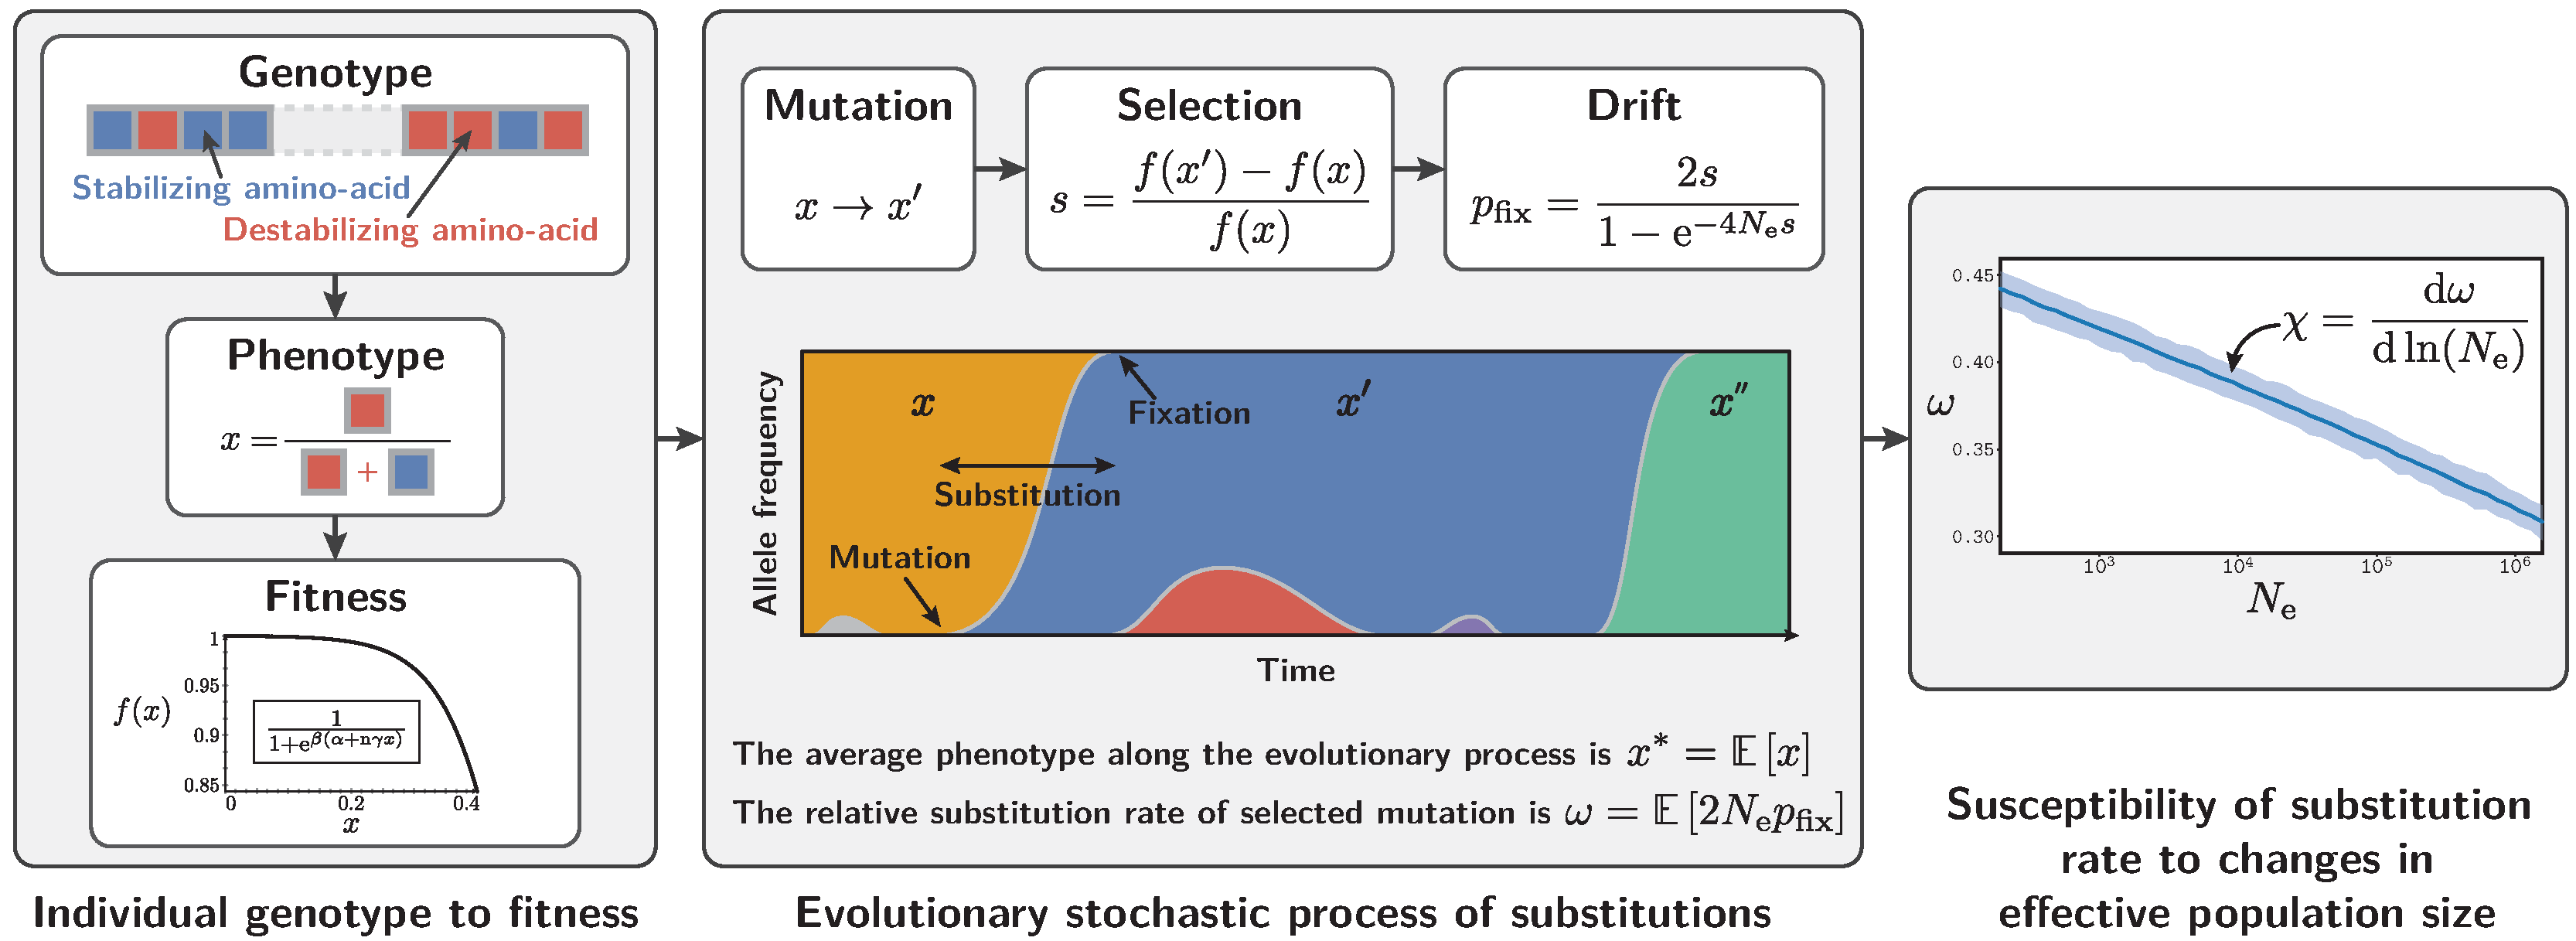
\includegraphics[width=\textwidth, page=1] {summary.pdf}
    \caption[Outline of the theoretical results]{
    Outline of the theoretical results.
    Left panel.
    The complete state of the amino-acid sequence is the genotype.
    The \gls{Phenotype} ($x$) is a real-valued summary of the genotype, and is defined in our model as the fraction of destabilizing sites in the sequence.
    Fitness is a decreasing log-concave function of the \gls{Phenotype}, depending on structural parameters of the model ($\Nsites, \DeltaGmin, \ \gamma, \ \beta$).
    Middle panel.
    Once defined the relation from genotype to fitness at the individual level, the evolutionary process consists of point \glspl{substitution} of the amino-acid representative sequence of the population.
    \Glspl{substitution} are mutation reaching fixation, thus the rate of \gls{substitution} depends mechanistically on the interplay between mutation, selection and \gls{drift}.
    For a given \gls{effective-population-size} ($\Ne$), the evolutionary process result in an average value of the \gls{Phenotype} ($\smash{x\eq}$) and an average relative \gls{substitution} rate of selected mutation ($\avgpfix$).
    Averaging over time is equivalent to determining the statistical equilibrium, by ergodicity of the stochastic process, given we can derive the probabilities of {transitions} between \glspl{Phenotype}.
    Right panel.
    The scaling of equilibrium $\avgpfix$ under a range of $\Ne$ give us the susceptibility ($\chi$), as a function of the structural parameters defined in the phenotype-fitness map.
    }
    \label{fig:Summary}
\end{figure}
In the original biophysical model, the protein stability is the difference in free energy between folded and unfolded conformations, called $\deltaG$ in kcal/mol.
Technically, free energy of the folded and unfolded conformations are computed based on the $3$D conformations of the protein and statistical potentials.
In such models, the stabilizing or destabilizing effect of an amino-acid at a particular site depends on amino acids present in the vicinity in $3$D conformation, taking into account specific epistasis~\citep{Dasmeh2018}.

We approximate this model such that destabilizing effect at a particular site does not depend on other neighboring residues, disregarding specific epistasis~\citep{Dasmeh2014}.
Instead, each site contributes independently to $\deltaG$.
With such approximation, for each site of the sequence only one amino-acid is stabilizing the protein.
All $19$ other amino acids are equally destabilizing, and each site contribute to an excess of $\gamma = \Delta \Delta G > 0$ (in kcal/mol) to $\deltaG$ per destabilizing amino acids.
If all amino acids of the sequence are stabilizing, $\deltaG$ is optimal and equal to $ \DeltaGmin = \Delta G_{\text{min}} < 0$.
In this model, the most succinct \gls{Phenotype} of a given genotype (i.e. sequence) is just the proportion of destabilizing amino acids in the sequence, defined as $0 \leq x \leq 1$.
Thus $\deltaG$ is a linear function of $x$:
\begin{align}
    \deltaG (x) = \DeltaGmin + \Nsite \gamma x,
\end{align}
where $\Nsite$ is the number of sites in the sequence.

For a given $\deltaG$, thermodynamic equations allows to derive the proportion of protein in folded conformation in the cytoplasm, which is assumed to be a proxy for fitness.
This fitness function is motivated in part that a protein must be folded to perform its function, however this a strong assumption which will be relaxed subsequently to take into account protein expression level.
Analytically, this fitness is given by Fermi Dirac distribution and is typically close to $1$, leading to a first-order approximation~\citep{Goldstein2011}:
\begin{align}
    \wrightfit (x) = \dfrac{1}{1 + e^{\beta (\DeltaGmin + \Nsite \gamma x)}},\\
    \Rightarrow \wrightfit (x) \simeq 1 - e^{\beta (\DeltaGmin + \Nsite \gamma x)},
\end{align}
where $\DeltaGmin$ and $\gamma$ are defined as above, and the parameter $\beta$ is $1.686$ mol/kcal at room temperature.

\subsection{Susceptibility of \texorpdfstring{$\avgpfix$}{φ} to changes in \texorpdfstring{$\Ne$}{Nₑ}. Analytical approximation}

In this section we present an analytical approximate solution for the response of equilibrium $\avgpfix$ after a change in $\Ne$ (in log space).
We call this response the susceptibility of $\avgpfix$ to changes in $\Ne$, and denote it as $\chi$:
\begin{align}
    \chi = \frac{ \der \avgpfix}{\der \ln (\Ne)} \label{eq:chi}
\end{align}
Broadly, deriving $\chi$ is done in two steps (See figure \ref{fig:Summary}).
First, we determine the \gls{Phenotype} at equilibrium, when evolutionary forces of mutation, selection and \gls{drift} compensate each other.
Subsequently, differential calculus on the response of the equilibrium \gls{Phenotype} to a change in $\Ne$ allows to ultimately derive an equation for $\chi$.
Main results are given in the general case of any phenotype-fitness map, and also derived in the specific case of the biophysical model, where the fitness is proportional to the total amount of folded protein.
All developments are available in supplementary materials in the most general case.

From a given genotype, mutations of its underlying sequence have various effects, they can increase or decrease the proportion of destabilizing amino-acid, or do nothing if the mutation is between two destabilizing amino acids.
To derive probabilities of such events to occur, we also make the simplifying assumption that all {transitions} between amino acids are equiprobable.
Altogether, any mutation in the sequence can then have a phenotypic effect of $0$ or $\dx=\sfrac{1}{\Nsite}$, with probabilities of {transition} equal to:
\begin{gather}
    \begin{cases}
        \dx &\text{ with probability } 1-x, \\
        0 &\text{ with probability } \frac{18 x }{19}, \\
        -\dx &\text{ with probability } \frac{x}{19}.\\
    \end{cases} \label{eq:proba}
\end{gather}
In the extreme case of an optimal \gls{Phenotype} ($x = 0$), only destabilizing mutations are proposed.
Moreover, the probability to propose a stabilizing mutation (effect $-\dx$), or in between destabilizing amino acids (effect $0$) is proportional to $x$.
Or in other words, mutation bias is proportional to $(1-x)/x$, which this is fundamentally a combinatorial effect, due to the number of mutational opportunities available in either direction.

Second, we need to determine the strength of selection acting on mutations.
Destabilizing mutations are selected against with a negative selection coefficient which can be approximated by:
\begin{align}
    s & \simeq \frac{1}{\Nsite}\frac{ \partial \logfit (x) }{\partial x} \label{eq:s} \\
    \Rightarrow s & \simeq - \beta \gamma e^{\beta (\DeltaGmin + \Nsite \gamma x)}, \label{eq:s-unfolded}
\end{align}
where $ \logfit = \ln \wrightfit$ is the log-fitness (or malthusian fitness).
Conversely, stabilizing mutations will be under positive selection with opposite sign but same absolute value.
It is important to realize that the selective effect is dependent on $x$, and that because the fitness function is log-concave, the absolute value of $s$ increases with regards to $x$.

Based on these expressions for mutational and selective pressure, one can study the evolutionary process trajectory.
Starting from an optimal sequence, mostly destabilizing mutations will occur, but they may reach fixation and accumulate until selection coefficients against new deleterious mutations is too strong, at which point the protein will reach a point of equilibrium called marginal stability~\citep{Taverna2002, Bloom2007}.
Most importantly the probability of fixation of mutations is affected by \gls{drift}, parameterized by \gls{effective-population-size} ($\Ne$).
Altogether, at the equilibrium between mutation, selection and drift, selection coefficients of new advantageous and deleterious mutations reaching fixations are expected to be null on average~\citep{Goldstein2013}.
Formally, and after simplification, the equilibrium \gls{Phenotype} denoted $x\eq$ is given in the general case by:
\begin{align}
    \ln \left( \frac{1 - x\eq}{x\eq} \right) + \ln (19) & \simeq - \frac{4\Ne}{\Nsite} \frac{ \partial \logfit (x\eq) }{\partial {x\eq}} \\
    \Rightarrow \ln \left( \frac{1 - x\eq}{x\eq} \right) + \ln (19) & \simeq 4\Ne \beta \gamma e^{\beta (\DeltaGmin + \Nsite \gamma x\eq)} \text{,} \label{eq:equilibrium}
\end{align}
in the more specific case of the biophysical model.
This equation essentially expresses the mutation-selection equilibrium: the left-hand side of the equation is the log of the mutation bias at $x$, while the right-hand side is simply $4 \Ne s$, the scaled selection coefficient.

This equation cannot be solved explicitly for $x\eq$, but a qualitative intuition on the consequences of change in $\Ne$ to the equilibrium \gls{Phenotype} $x\eq$ is given in figure \ref{fig:NeChangeInfluence}.
Intuitively an increase in $\Ne$ results in a more optimal \gls{Phenotype}, closer to $0$.
Mutation bias (left-hand side of equation \ref{eq:equilibrium}) decreases with $x$ while the strength of selection (right-hand side of equation \ref{eq:equilibrium}) increases with $x$, and the equilibrium \gls{Phenotype} is obtained at their intersection.
An increase in $\Ne$ (green dotted curve) leads to shifting the selective response upward, which then results in a leftward shift of the equilibrium \gls{Phenotype}, closer to $0$.
The leftward shift is smaller for selective strength with steeper curve, resulting in qualitatively weaker susceptibility of the equilibrium \gls{Phenotype} to changes in $\Ne$

\begin{figure}[H]
    \centering
    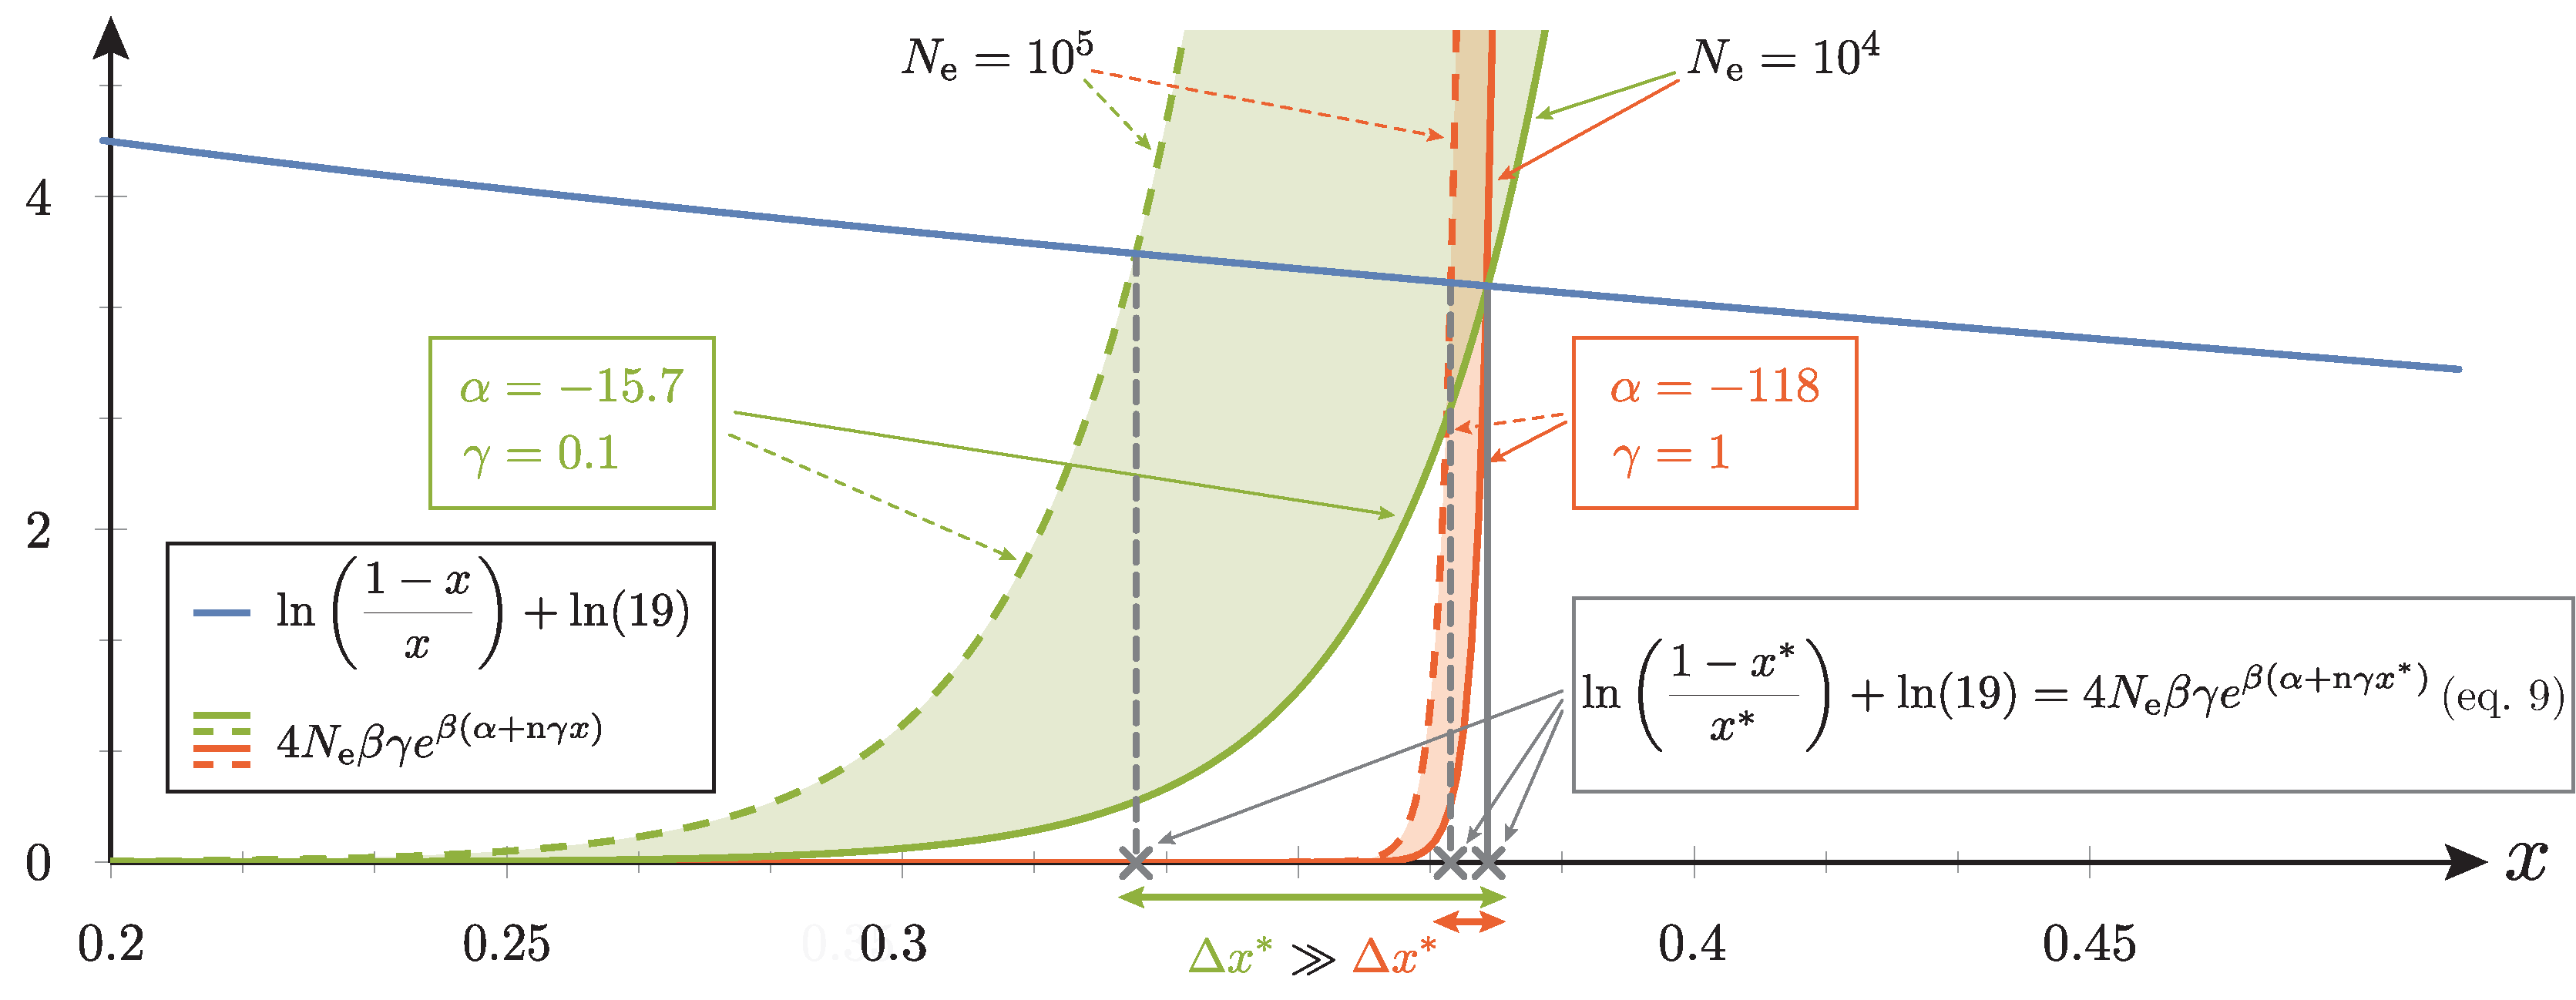
\includegraphics[width=\textwidth, page=1] {theoretical.pdf}

    \caption[Phenotype susceptibility after a change in $\Ne$]{
    Phenotype susceptibility after a change in $\Ne$.
    The equilibrium \gls{Phenotype} $x\eq$ is determined by the equation $\smash{\ln(\frac{1 - x\eq}{x\eq}) + \ln(19)=4\Ne \beta \gamma e^{\beta (\DeltaGmin + \Nsite \gamma x\eq)}}$.
    The right-hand side of the equation increases exponentially with $x$ where $\Nsite \gamma$ is the exponential growth rate ({\color{RED}red} and {\color{GREEN}green} curves).
    The parameter $\gamma$ is chosen such that $\gamma$ is increased by an order of magnitude in the red compared to the green curve, moreover, the value of $\DeltaGmin$ is chosen such that the equilibrium value $\smash{x\eq}$ is kept constant by solving numerically equation \ref{eq:equilibrium}.
    Whenever $\Nsite \gamma$ is large ({\color{RED}red solid} curve), the exponential growth is steep and increasing $\Ne$ (dotted curve) only changes subtly the equilibrium \gls{Phenotype} by a factor $\smash{\color{RED}\Delta x\eq}$.
    On the other hand, whenever $\Nsite \gamma$ is low ({\color{GREEN}green} solid curve), the exponential growth is steadier and increasing $\Ne$ (dotted curve) involve a stronger susceptibility of the equilibrium \gls{Phenotype} by a factor $\smash{\color{GREEN}\Delta x\eq}$.
    Moreover, changes in $\smash{x\eq}$ reflects the changes in $\avgpfix$ since both are approximately equal (equation \ref{eq:dnds}).
    }
    \label{fig:NeChangeInfluence}
\end{figure}

Results thus far ties only equilibrium \gls{Phenotype} ($x\eq$) to $\Ne$.
To capture how $\avgpfix$ varies with $\Ne$, we also need to obtain an expression for $\avgpfix$ as a function of $x\eq$.
At equilibrium we can derive (supplementary materials) the expected \gls{substitution} rate of mutations changing the amino-acid sequence, and by normalizing by the \gls{substitution} rate of \gls{neutral} mutations, $\avgpfix$ simply approximates to:
\begin{gather}
    \avgpfix \simeq x\eq \label{eq:dnds}
\end{gather}
This simple approximation is due to \glspl{substitution} at destabilizing sites (proportion $x\eq$) to one of the other destabilizing amino acids, which are effectively \gls{neutral} and compose the largest proportion of proposed mutations with substantial probability of fixation (equation \ref{eq:proba}).

Taken together, implicit derivation of the equilibrium with regards to $\Ne$ yields the susceptibility (equation \ref{eq:chi}) of $\avgpfix$ to a change in $\Ne$:
\begin{gather}
    \chi = \frac{ \der \avgpfix}{\der \ln (\Ne)} \simeq - \frac{\frac{ \partial \logfit (x\eq) }{\partial {x\eq}}}{\frac{\Nsite}{4 \Ne} \frac{\partial \ln [ (1 - x\eq) / x\eq ]}{\partial x\eq } + \frac{ \partial^2 \logfit (x\eq) }{\partial {x\eq}^2}}.
\end{gather}
The two terms of the denominator correspond to the derivative of respectively the mutational bias and scaled selection coefficient.
However, mutational bias decreases weakly with $x$ (blue curve on figure \ref{fig:NeChangeInfluence}) while the strength of selection increases sharply with $x$ (red and green curves).
As a consequence, the \gls{Phenotype} is not equimutable, meaning the mutational bias is not constant, but nearly so since the derivative of the mutational bias is greatly lower than the derivative of the selection coefficient around the equilibrium point.
This simplification lead to a very compact equation for susceptibility $\chi$ in the general case:
\begin{gather}
    \chi \simeq - \frac{\frac{ \partial \logfit (x\eq) }{\partial {x\eq}}}{\frac{ \partial^2 \logfit (x\eq) }{\partial {x\eq}^2}}
\end{gather}
Susceptibility is thus equal to the inverse of the relative curvature, i.e. the ratio of the second to the first derivatives, of the log-fitness function, taken at the equilibrium \gls{Phenotype}.
Of note, this susceptibility is strictly negative for decreasing log-concave fitness functions, asserting that $\avgpfix$ is a decreasing function of $\Ne$.
In addition, susceptibility itself is low (i.e. $\avgpfix$ responds more weakly) for strongly concave log-fitness functions, thus quantitatively capturing the intuition developed in figure \ref{fig:NeChangeInfluence}, explicitly that the amount of change on $\avgpfix$ is very small if the selection coefficient curve is very steep around the equilibrium set point (red curve compared to green curve).

In the specific case of the biophysical model, the susceptibility ($\chi$) further simplifies to:
\begin{gather}
    \chi \simeq -\dfrac{1}{\beta \Nsite \gamma}, \label{eq:chi_application}
\end{gather}
Meaning that $\avgpfix$ is linearly decreasing with $\Ne$ (in log scale) since $\chi$ is independent of $x\eq$, or, in other words, the exact value of the equilibrium \gls{Phenotype} has no impact on the slope.
Moreover, only the compound parameter $\beta \gamma \Nsite$ has an impact on the slope of the linear relationship.
In practice, the structural and molecular parameters of the model are $\DeltaGmin = \Delta G_{\text{min}}$ and $\gamma = \Delta \Delta G$ such that the slope of the linear relationship between $\avgpfix$ and $\Ne$ is affected by $\Delta \Delta G$ but not by $\Delta G_{\text{min}}$.
Importantly, only relative values of $\Ne$ (multiplicative) and $\avgpfix$ (additive) are sufficient to estimate empirical value of $\chi$, absolute values are not necessary.
% Although the general equation seems to suggest in appearance that elasticity only depends on the fitness function, in fact, what the biophysical model shows is that the elasticity can actually be modulated in two ways: by playing on the genotype / \gls{Phenotype} relationship (here, $\gamma$), or by playing on the fitness \gls{Phenotype} relationship (here, beta). All the more reason to consider beta as a potentially free parameter too.

\subsection{Susceptibility of \texorpdfstring{$\avgpfix$}{φ} to changes in protein expression level}

\label{sec:expression}

Effective population size is not the sole predictor of $\avgpfix$, and expression level (or protein abundance) is also negatively correlated to $\avgpfix$.
Our previous model, however, does not express the fact that selection is typically stronger for proteins characterized by higher levels of expression.
Nonetheless, our previous general equations can be directly applied when we assume that each misfolded protein has the same relative effect on fitness~\citep{Drummond2005a, Wilke2006, Drummond2008, Serohijos2012}.
For a given protein with expression level $y$ and a cost $c$ per misfolded macromolecule, the fitness and selective coefficient are defined as follow, leading to the mutation-selection-drift equilibrium:
\begin{gather}
    \logfit (x) \simeq - c y e^{\beta (\DeltaGmin + \Nsite \gamma x)} \\
    \Rightarrow s \simeq - \beta \gamma c y e^{\beta(\DeltaGmin + \gamma \Nsite x)} \\
    \Rightarrow \ln \left( \frac{1 - x\eq}{x\eq} \right) + \ln (19) = 4\Ne y A \beta \gamma \Nsite e^{\beta(\alpha + \gamma \Nsite x\eq)}
\end{gather}
Importantly, $\Ne$ and $y$ are confounded factors in the mutation-selection-drift equilibrium equation, both appears only once and they are multiplied.
This means that increasing either $\Ne$ or $y$ leads to same change in equilibrium \gls{Phenotype}, hence the same $\avgpfix$, and ultimately the same susceptibility:
\begin{align}
    \chi = \frac{ \der \avgpfix\eq}{\der \ln (\Ne)} = \frac{ \der \avgpfix\eq}{\der \ln (y)} \simeq - \frac{1}{\beta \Nsite \gamma}. \label{eq:chi_application_y}
\end{align}
Equation \ref{eq:chi_application_y} can also be proven under more general hypothesis relating \gls{Phenotype} to fitness, for example if the selective cost is due to translational errors.
If the protein is assumed to be regulated such as to reach a specific level of functional proteins abundance under a general cost-benefit argument~\citep{Cherry2010,Gout2010}, a multiplicative factor depending solely on the expression level is prefixed (see supplementary materials).
Altogether, we theoretically obtain the same linear decrease of $\avgpfix$ w.r.t either \gls{effective-population-size} or expression level (in log space) under a broad variety of hypothesis.

\subsection{Simulation experiments}

Our theoretical derivation of the susceptibility of $\avgpfix$ to changes in $\Ne$ (and expression level) is based on several simplifying assumptions about the evolutionary model and makes multiple approximations.
In order to test the robustness of our main result, we therefore conducted systematic simulation experiments, relaxing several of these assumptions.
In each case, simulations were conducted under a broad range of values of $\Ne$, monitoring the average $\avgpfix$ observed at equilibrium and plotting the scaling of these measured equilibrium $\avgpfix$ as a function of $\Ne$.

Specifically, with respect to mutations, our derivation assumes that all amino-acid {transitions} are equiprobable, in other words, the complexity of the genetic code is not taken into account.
Simulating evolution of \acrshort{DNA} sequence, and taking into account a matrix a mutation rate between nucleotide allows to test directly the robustness of the results to this assumption.
Furthermore, with regard to the phenotypic effects of amino-acid changes, we previously assumed that all destabilizing amino acids are having an identical impact on protein stability.
In reality, one would expect conservative amino-acid replacements to be less destabilizing than radical changes.
This assumption is relaxed in our simulation, such that destabilizing mutations in each position are now proportional to the Grantham distance~\citep{Grantham1974} between the optimal amino-acid in this position and the amino-acid proposed by the non-synonymous mutation.
Additionally, the number of sites in the sequence ($\Nsite$) is assumed to be large such that the selection coefficient is well approximated by the fitness derivative (equation \ref{eq:s}).
The robustness of such approximation is tested in the simulations with finite sequences ($\Nsite=300$).
% Finally, the \gls{substitution} rate is known to vary among sites within a protein, and each site does not contribute equally to the stability of the protein~\citep{Echave2016}.
% To mimic this effect, the destabilizing effect of mutations is scaled by a factor specific to each site, drawn from gamma distribution (see supplementary materials).

Simulations demonstrate that the relation between $\avgpfix$ and log-$\Ne$ is indeed linear, at least in the range explored here, and that the slope of the linear regression matches the expected theoretical value (figure \ref{fig:GoldsteinVsToy}A).
Secondly, we observe that the parameter $\DeltaGmin$ has virtually no effect on the slope of the linear regression, as also expected theoretically (figure \ref{fig:GoldsteinVsToy}B).
Instead, decreasing $\DeltaGmin$ (to more negative values) merely results in an overall increase in $\avgpfix$ over the whole range of $\Ne$ (i.e. has an impact on the intercept, not on the slope).
This is due to the fact that decreasing $\DeltaGmin$ shifts the equilibrium to higher $x\eq$, since more destabilizing sites can then reach fixation before reaching the point of marginal stability.

Finally, we relaxed our assumption that each site of the sequence contributes independently to $\deltaG$, by taking into account the $3$D structure of protein and using a statistical potential to estimate $\deltaG$.
We implemented the original model~\citep{Williams2006, Goldstein2011, Pollock2012}, in which the free energy of the folded are unfolded conformations are computed using $3$D structures of the protein conformations and pairwise contact potential energies between neighboring amino-acid residues~\citep{Miyazawa1985} (supplementary materials).
The original works showed that under such $3$D model, $\avgpfix$ is approximately independent of $\Ne$~\citep{Goldstein2013}.
Using extensive simulations in order to obtain sufficient resolution, we observe that $\avgpfix$ is in fact weakly dependent on $\Ne$, being approximately linear with log-$\Ne$ (figure \ref{fig:GoldsteinVsToy}C).
Moreover, the observed slope matches the theoretical value considering $\deltadeltaG = 1.0$ kcal/mol for destabilizing mutations and $\Nsite=300$.
In such experiment, $\DeltaGmin=-118$ kcal/mol as it is the $\deltaG$ of the optimal sequence of $300$ sites~\citep{Goldstein2011} (figure \ref{fig:GoldsteinVsToy}D).
\begin{figure}[H]
    \centering
    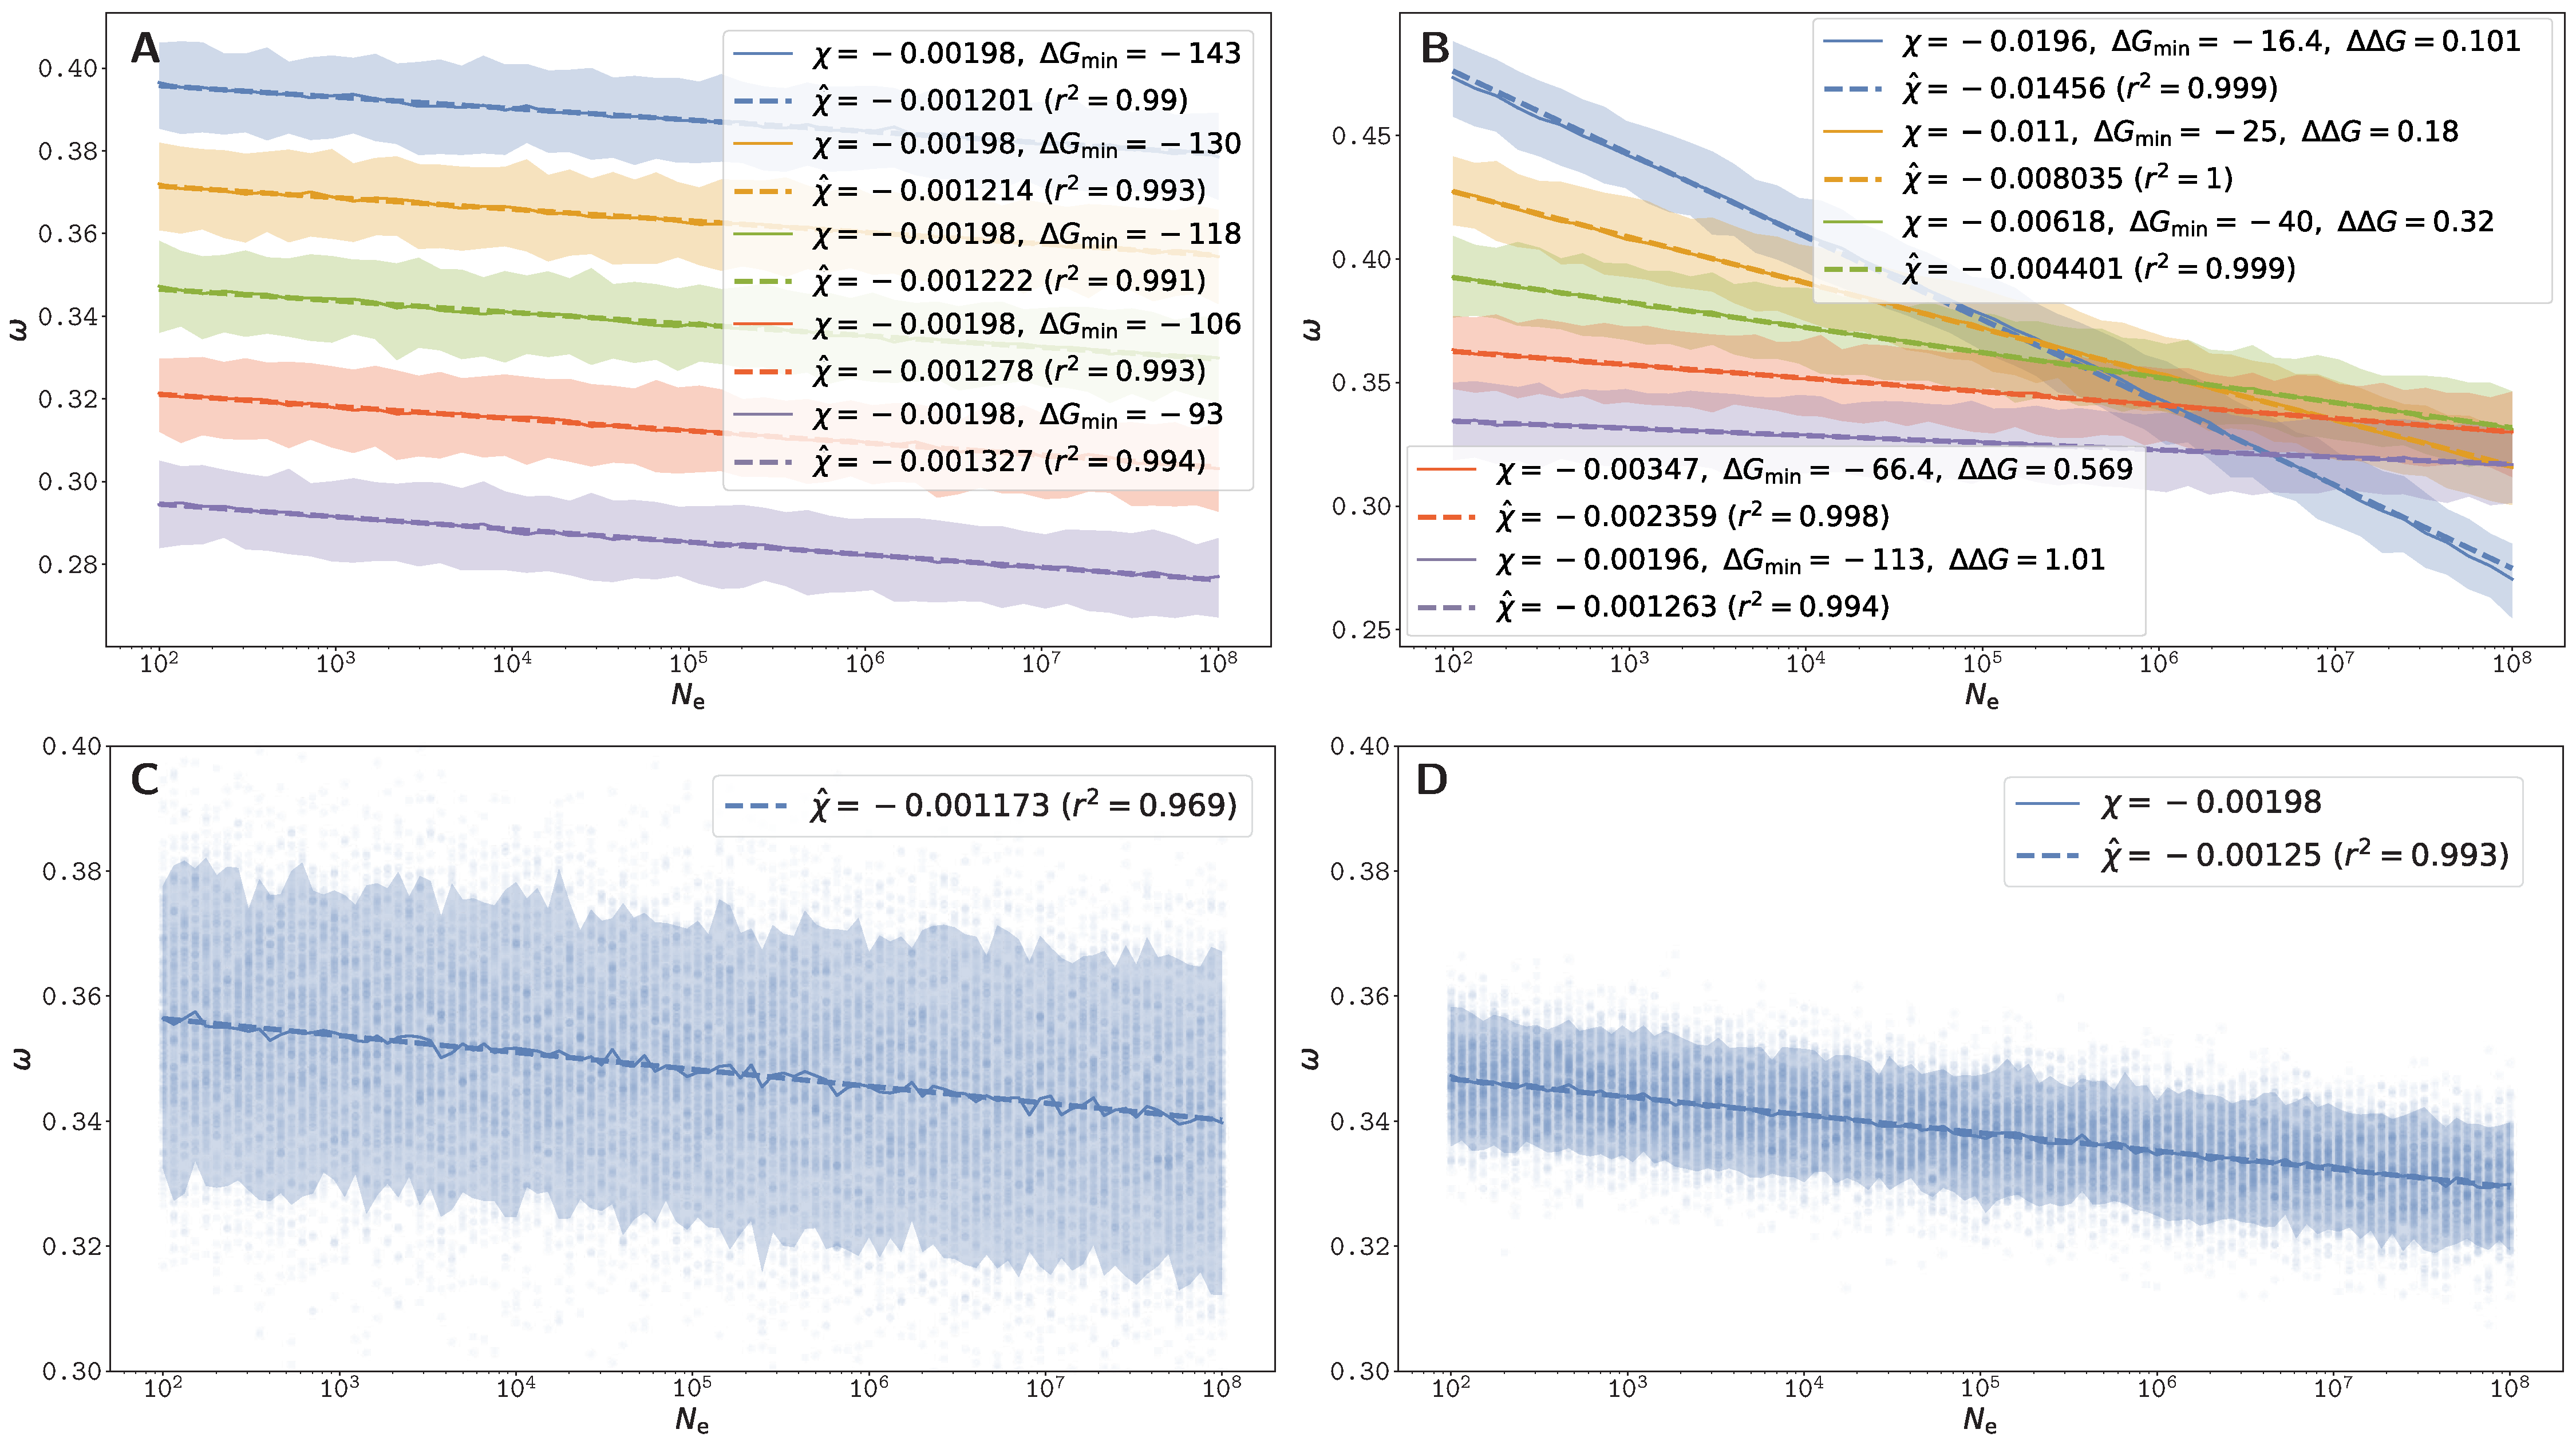
\includegraphics[width=\textwidth] {elasticity-low.pdf}

    \caption[$\avgpfix$ susceptibility to change in $\Ne$]
    {$\avgpfix$ susceptibility to change in $\Ne$.
    Scaling experiment simulating sequence evolution and recording the average $\avgpfix$ (y-axis) observed at equilibrium as a function of $\Ne$ (x-axis).
    Along the x-axis, $200$ replicate simulations are performed for each different $\Ne$, the average (solid lines) and $90\%$ confidence interval (shaded area) of $\avgpfix$ are shown.
    Linear regression (dashed lines) allows to estimate the susceptibility ($\hat{\chi}$), which is compared to theoretical expectation.
    The fixed parameters are $\Nsite=300$, $\beta=1.686$.
    Simulations are conducted under our additive \gls{Phenotype} model (expect panel C), and for each non-optimal amino-acid $\gamma$ is scaled by the Grantham distance to the optimal amino-acid.
    Panel A; $\DeltaGmin$ and $\gamma$ are given in the legend.
    $\gamma$ is increased and $\DeltaGmin$ is changed accordingly such that the equilibrium value $\smash{x\eq}$ is kept constant, by solving numerically equation \ref{eq:equilibrium}.
    The estimated susceptibility ($\hat{\chi}$) decreases proportionally to the inverse of $\gamma$, as predicted by our theoretical model.
    Panel B; $\gamma=1$ and $\DeltaGmin$ are given in the legend.
    Decreasing $\DeltaGmin$ (to more negative values) increases $\avgpfix$ but changes hardly the slope of the linear regression, as expected theoretically.
    Panel C; Folding free energy that determines the stability of the folded native state is computed using $3$D structural conformations and pairwise contact potential energies between neighboring amino-acid residues.
    The estimated susceptibility $\hat{\chi}=0.00124$, and $\avgpfix$ at equilibrium is weakly dependent on log-$\Ne$, but not completely as originally claimed~\citep{Goldstein2013}.
    Under the approximation of an additive free energy model and with empirical estimate of $\gamma = \Delta \Delta G \simeq 1$, our theoretical prediction is $\chi = 0.00198$, close to the observation using $3$D structural conformations.
    Panel D; structural parameters are matched to their empirical estimates of $\DeltaGmin=\Delta G_{\text{min}} = -118$ and $\gamma = \Delta \Delta G = 1$.
    Under such parametrization, the scaling behavior is similar to panel C, although with less variance.
    \label{fig:GoldsteinVsToy}
    }
\end{figure}

\subsection{Time to relaxation}

Although the equilibrium value of $\avgpfix$ after changes in $\Ne$ is an important feature of the $\avgpfix$-$\Ne$ relationship, another characteristic that is scarcely studied is the dynamic aspect~\citep{Jones2016}, particularly the relaxation time to reach the new equilibrium $\avgpfix$.
We observed in our simulations that the determining factor of the relaxation time is the number of sites $\Nsite$ (figure \ref{fig:relaxStability}A), such that the return to equilibrium is faster for longer sequences.
These observations match the theoretical prediction that more mutational opportunities are available for longer sequences, driving the trait close to equilibrium at a faster rate.

It may be useful to compare the relaxation pattern observed here with the predictions under two alternative models of sequence evolution, representing two extreme scenarios.
On one hand, having fitness modeled at the level of sites, such as those contemplated by many phylogenetic mutation-selection models~\citep{Halpern1998, Rodrigue2010, Tamuri2012}, thus every site has to adapt on its own to the new change in $\Ne$.
The relaxation time is very long, on the order of the inverse of the per-site \gls{substitution} rate.
On the other hand, assuming a fixed distribution of fitness effect (\acrshort{DFE}), the response of $\avgpfix$ is instantaneous (figure \ref{fig:relaxStability}B).
Our model is effectively in between these two extreme scenarios.

Another characteristic observed is the non-continuity of $\avgpfix$ after a change in $\Ne$.
Both an increase and decrease in $\Ne$ lead to a discontinuity in $\avgpfix$.
Most importantly $\avgpfix$ is suddenly higher regardless of the change's direction in $\Ne$, then smoothly reaching the equilibrium value (figure \ref{fig:relaxStability}A \& \ref{fig:relaxStability}B).
Similarities in these non-equilibrium properties can both be explained mechanistically.
Under low $\Ne$, the \gls{Phenotype} is far away from the optimal \gls{Phenotype} because the strength of selection is weaker.
A sudden increase in $\Ne$ result first in a short traction toward a more optimal \gls{Phenotype}, which can results into suddenly higher $\avgpfix$, seemingly to an adaptation.
Conversely, under high $\Ne$ the \gls{Phenotype} is closer to optimal and the purification of deleterious mutations is stronger.
The reaction to a decrease in $\Ne$ is a relaxation of the purification and thus a $\avgpfix$ closer to the \gls{neutral} case, which results into higher $\avgpfix$ until the point of marginal stability.
To note, an increase in $\Ne$ can theoretically and possibly lead to a temporarily $\avgpfix > 1$ due to adaptive evolution~\citep{Jones2016}, while an decrease in $\Ne$ always imply $\avgpfix < 1$ due to at most a \gls{neutral} regime of relaxed selection.
\begin{figure}[H]
    \centering
    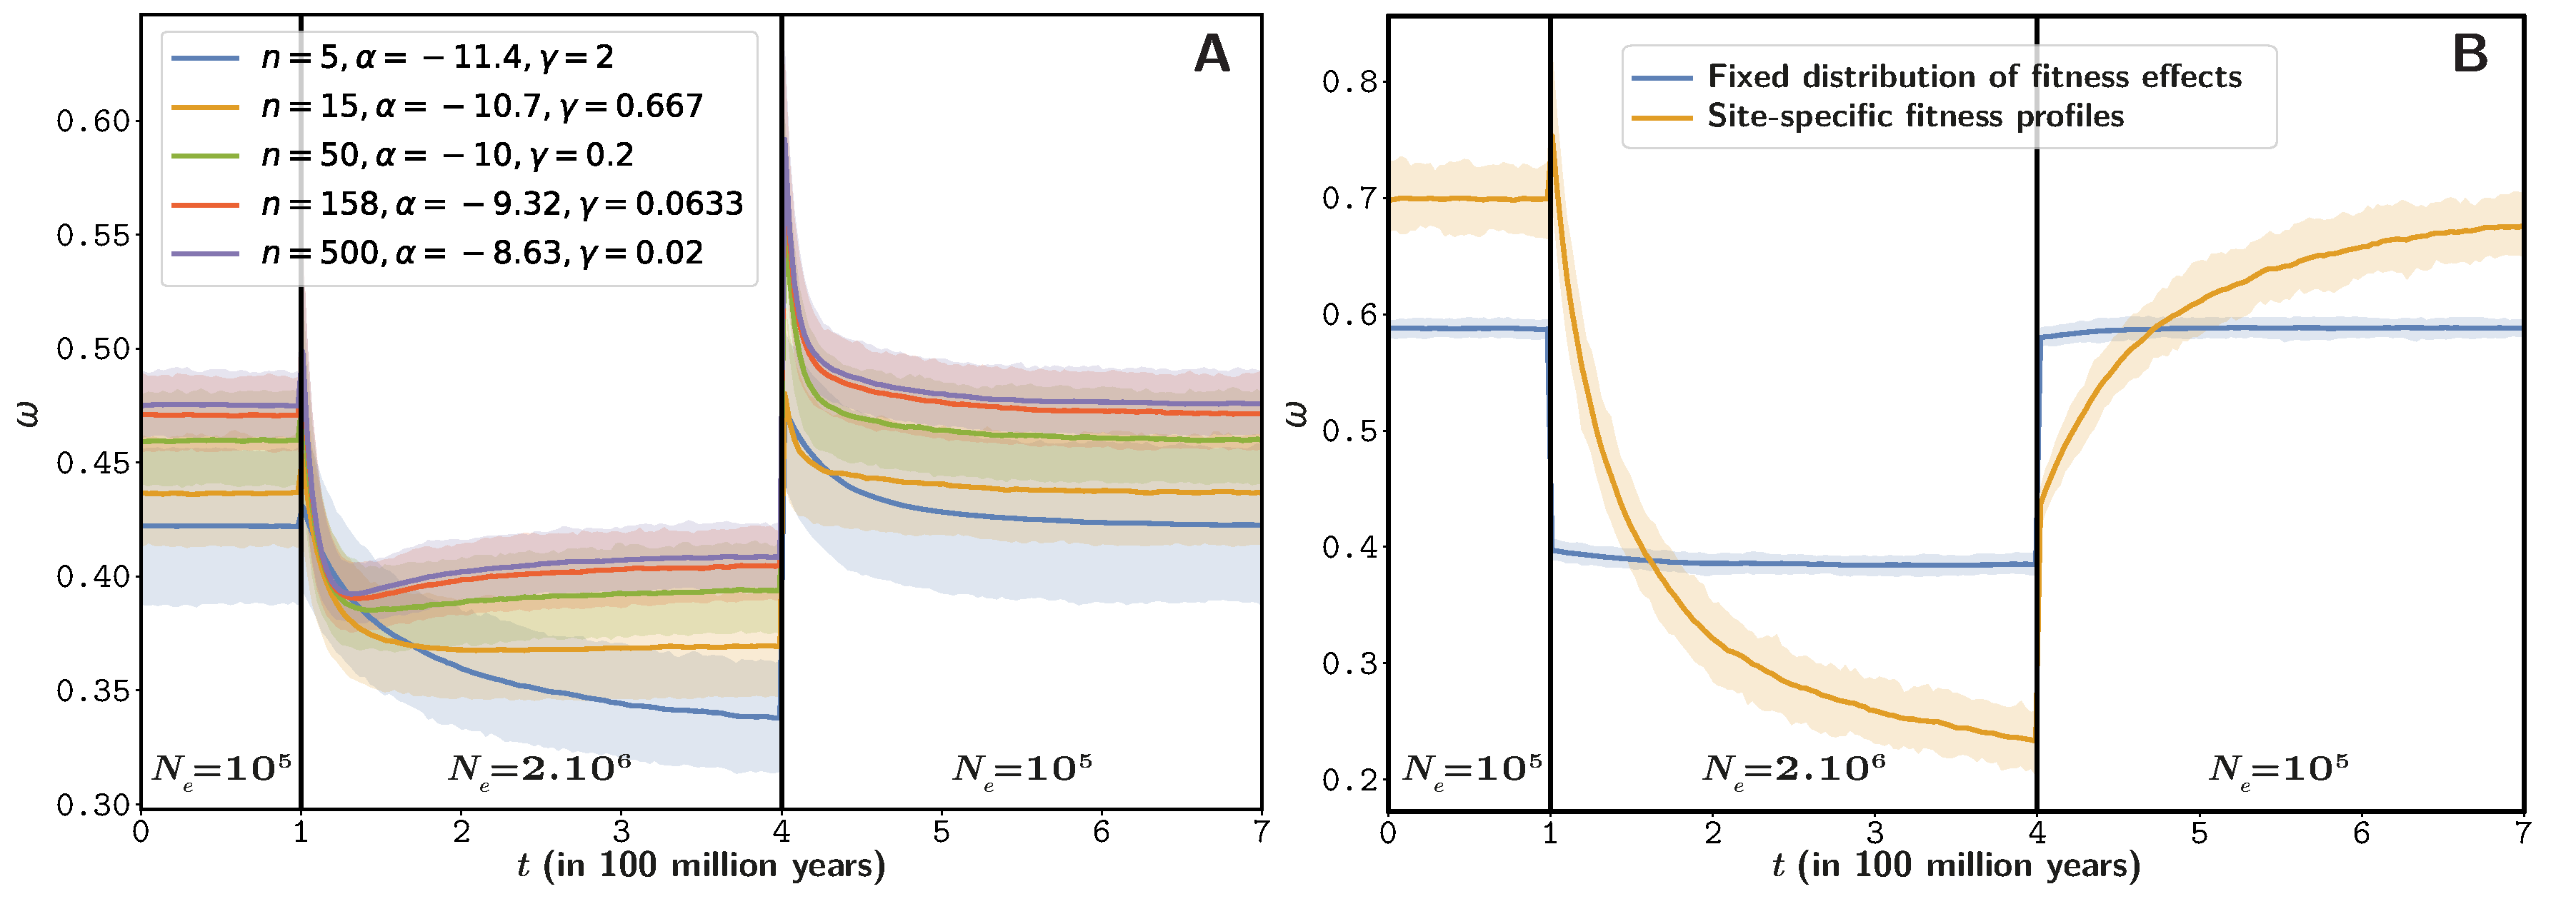
\includegraphics[width=\textwidth] {Relaxation.pdf}

    \caption[ $\avgpfix$ relaxation after a change in $\Ne$]{
    $\avgpfix$ relaxation after a change in $\Ne$.
    Solid line corresponds to the average over $1000$ replicates and the shaded area correspond to the $90\%$ interval among replicates.
    The mutation rate ($\mu$) is $1e{-8}$ per year per site, and the total time of the computation is $700$ million years.
    Panel A.
    $\beta=1.686$ for all simulations.
    The \acrshort{DNA} sequence of $500$ sites is divided into exons of equal size.
    However the number of sites per exon changes between simulations from $\Nsite=5$ to $\Nsite=500$.
    Moreover, $\gamma$ is changed according to the exon size such that the product is kept constant, and as a consequence the susceptibility of $\avgpfix$ to changes in $\Ne$ is kept constant.
    Finally, $\DeltaGmin$ is changed accordingly such that the equilibrium value $\smash{x\eq}$ is kept constant, by solving numerically equation \ref{eq:equilibrium}.
    As such, whatever the exon size, $\smash{x\eq}$ and $\chi$ are kept constant and thus the observed effect is due to the number of sites in the exon.
    We observe that increasing the number of sites implies a reduced time to reach the new equilibrium.
    Panel B.
    In context of a fixed fitness landscape, where each amino-acid has different fitness (site-specific profile), the time taken to reach the new equilibrium value of $\avgpfix$ after a change in $\Ne$ is long, such that relaxation rate is on the order of the mutation rate.
    In the context of a fixed distribution of fitness effects (\acrshort{DFE}), the relaxation time is non-existent and the new equilibrium value of $\avgpfix$ is reached instantaneously.
    }
    \label{fig:relaxStability}
\end{figure}


\section{Discussion}
% Goal and theoretical results

We provide a compact analytical result for the equilibrium response of $\avgpfix$ to changes in $\Ne$, and relate this response to the parametrization of the genotype-phenotype-fitness map.
An application to selection against protein misfolding prove that the susceptibility of $\avgpfix$ to variation in $\Ne$ (in log space) is linear with a negative slope.
Furthermore, this application demonstrate that \gls{effective-population-size} and protein expression level are interchangeable in respect to their impact on the response of $\avgpfix$.
Overall, the susceptibility ($\chi$), is a function of structural parameters of the protein, and is inversely proportional to the product of three terms; namely the sequence size, the inverse temperature ($\beta$), and the average change in conformational energy of destabilizing mutations ($\Delta \Delta G$).
This product can be several orders of magnitude greater than $1$ in practice, such that the susceptibility of $\avgpfix$ is its inverse, very subtle and weak.

%The negative relationship between the relative \gls{substitution} rate of selected mutations ($\avgpfix$) and the \gls{effective-population-size} ($\Ne$) has been predicted theoretically under the quasi-neutral theory of evolution.
%Empirical data showed mitigated confirmation of this prediction, encouraging alternative explanatory mechanism.
%One such explanation, developed in the context of genotype-phenotype-fitness map, demonstrated the absence of $\avgpfix$ susceptibility to changes in $\Ne$ if the probabilities of \gls{Phenotype} changes are invariant to the current \gls{Phenotype}.
%We argue that this assumption can be relaxed, and provide theoretical tools to derive the relationship between $\avgpfix$ and $\Ne$ at equilibrium in this context.
%We apply our framework in the special case of fitness proportional to the proportion of folded proteins.

Our compact theoretical results are supported by more complex simulations of protein evolution relaxing several assumptions.
Particularly, our theoretical prediction match a numerical model of protein evolution, in which the free energy of the folded and unfolded conformations are computed using $3$D structures of the protein conformations.
Previous studies using this model presented an apparent lack of $\avgpfix$ susceptibility to changes in $\Ne$~\citep{Goldstein2013}.
We argue the apparent lack of susceptibility is in fact due to a very subtle and weak relation, and require extensive computation to be detected.
Based on empirical estimate of the structural parameters $\beta = 1.686$, $\Nsite=300$ sites and $\gamma=\Delta \Delta G = 1.0$ kcal/mol~\citep{Zeldovich2007}, estimated susceptibility is $\hat{\chi} \simeq -0.002$.
In other words, for a relative increase in $\Ne$ or expression level of $6$ orders of magnitude, a factor approximately equal $0.01$ is subtracted to $\avgpfix$, a subtle relationship that requires laborious effort to be detected in simulated data.

To note, the models consider $\avgpfix$ across the entire protein and neglect variation among sites, which are not the focus of the analysis.

\subsection{Adequacy to empirical data}
Empirically, variation in $\avgpfix$ along the branches of phylogenetic trees has been inferred and correlated to proxies of $\Ne$, such as body size or other life-history traits.
These promising results showed mitigated confirmation of a negative $\avgpfix$ susceptibility to changes in $\Ne$~\citep{Lanfear2014}.
More recently, phylogenetic integrative methods refined the estimate of covariation between$\avgpfix$ and $\Ne$ along lineages by leveraging polymorphism data and genetic diversity of supposedly \gls{neutral} site, such as to estimate $\Ne$ by taking into account confounding factors~\citep{Brevet2019}.
These methods can give an estimate of $\hat{\chi} \simeq 0.02$ (see supplementary materials) at least one order of magnitude times greater than our theoretical prediction.
More empirical data across different clades would be required to robustly consolidate such empirical observation, but as of yet are challenging our theoretical predictions.

% Stress the importance that susceptibility is valid for Ne and protein abondance
Conjointly, the theoretical prediction of a weak negative $\avgpfix$ susceptibility to changes in protein expression level is in stark contrast with various empirical studies~\citep{Duret2000, Rocha2004, Wang2011, Song2017}.
Furthermore, protein expression level is one of the best predictors of $\avgpfix$ and the empirical estimation of $\chi$ in fungi, archaea and bacteria varies in the range $[-0.046;-0.021]$ (table in supplementary materials) extracted from \citet{Zhang2015}, which is in the best case one order of magnitude times greater than our theoretical prediction ($\simeq -0.002$).
Interestingly, estimation of $\chi$ in animals and plants varies in the range $[-0.026;-0.004]$, which is closer to theoretical estimate (table in supplementary materials).
Altogether, fitness based on protein stability is a compelling model of molecular evolution, but is apparently not a sufficiently comprehensive model to explain the amplitude of variation of $\avgpfix$ empirically observed along a gradient of either \gls{effective-population-size} or protein expression level.
Our theoretical work aligned with recent independent empirical studies providing negative evidence for the hypotheses linking the rate of sequence evolution with the toxicity constraint\citep{Plata2017,Razban2019,Biesiadecka2020}.

% Protein-protein interactions
Notably, the response of $\avgpfix$ to changes in expression level has also theoretically been found to arise due to protein interactions with the proteome, where protein may either be in free form or engaged in non-specific interactions~\citep{Yang2012, Zhang2013}.
In non-specific interactions at the protein surface, stabilizing amino acids are hydrophilic and destabilizing amino acids are hydrophobic, sticking to hydrophobic residues in other proteins~\citep{Dixit2013,Manhart2015}.
Our theoretical results can be applied more broadly to protein-protein interactions using a mean-field argument (supplementary materials).
Fitting this model with empirical structural estimates~\citep{Janin1995a, Zhang2008}, we obtain a susceptibility of $\chi \simeq -0.2$ thus a much stronger response than under the model based on conformational stability.
This effect is due to fewer sites in the protein being involved in protein-protein interaction than for conformational stability, in addition to lower energy engaged in contacts between residues.

Taken together, the assumption that protein fitness is in part determined such as to avoid non-specific interaction, instead of being determined by its probability of folding, leads to a stronger susceptibility of $\avgpfix$ to changes in $\Ne$ or protein expression level.
In conclusion, models of molecular evolution of the protein taking into account destabilizing effect protein-protein interactions, appears to be more compatible with empirical data obtained in comparative genomics, at least in the light of the susceptibility of $\avgpfix$ to changes in $\Ne$ or expression level.

\subsection{Physically grounded modeling}
% Analogy to physics
This study describes the signature imprinted on \acrshort{DNA} sequences by an evolutionary process by merging equations from population-genetics and from structural physico-chemical first principles.
Hence, physico-chemical vocabulary and theory are recruited to describe the molecular details.
More widely, our modeling is imprinted with vocabulary and analogy to physical systems, with wording in the likes of forces, susceptibility and dynamic.
We argue analogy between evolutionary and physical system is not restricted to wording, but allows to visualize and intuit of the causality chains and which approximation can be made such as to derive analytical tractable results~\citep{Sella2005, Mustonen2009, Bastolla2012, Bastolla2017}.
Because it is constructive approach, and not solely intuitive, the robustness of theoretical results to approximations can be asserted by computational implementation.
Computational models offer a means to test the validity and robustness, while mathematical models offer an intuitive mechanistic mental analogy.

% Thermodynamic analogy
% Analogy to Clapeyron formula ? TdP/dT = ΔH/ΔV, where T is analogous to Ne
A first analogy between evolutionary biology and physics comes from statistical mechanics, describing how observable macroscopic properties are emerging from microscopic states.
As an example, in the Ising model the magnetization is a macroscopic resultant of all microscopic atomic spins that can be in one of two states~\citep{Brush1967}.
At equilibrium when system reaches minimum potential energy, the observable magnetization is controlled by variable such as temperature, and by external forces such as a magnetic field forcing the system.
By analogy, our atoms are sites of the sequence which can be in stabilizing or destabilizing state, and the macroscopic emerging observable is the relative \gls{substitution} rate of selected mutation ($\avgpfix$), which is controlled by \gls{effective-population-size} ($\Ne$) analogous to temperature~\citep{Sella2005}.
Ultimately, the susceptibility of macroscopic observable ($\avgpfix$) to a control variable ($\Ne$) can be tied to the microscopic parameters.
Another example of observable macroscopic property, though not considered in this manuscript, could be for example site entropy, i.e. the effective number of observed amino-acid at equilibrium~\citep{Goldstein2016, Jimenez2018, Jiang2018}.

% Mechanical analogy
% Elasticity with springs ? Surface tension with molecule and radius of the
% Elasticity ? Susceptibility (dimensionless) ? Compliance (units of metres per newton) ? Flexibility (units of metres per newton) ?
A second analogy between evolutionary biology physics comes from mechanics, where \gls{Phenotype} represent a spatial coordinate of the system, which is determined by external evolutionary forces; namely mutation, selection and drift.
These evolutionary forces are analogous to springs attached and stretching the \gls{Phenotype} in various directions and with various stiffness, resulting in an equilibrium point.
Once the equilibrium point determined, an elastic (or reversible) deformation of the \gls{Phenotype} can be studied whenever applying a differential stress to the system.
In this analogy, changing the free energy of the reference \gls{Phenotype} ($\DeltaGmin = \Delta G_{\text{min}}$) leads in first approximation to changes of reference and equilibrium point but not a change in the stiffness of the springs, meaning the elastic coefficient (analog to susceptibility) is approximately conserved.
Conversely, stiffness ot the springs increases with regards to $\gamma = \Delta \Delta G$, meaning a that change in the stress applied to the system ($\Ne$) result in a weak deformation at the new equilibrium.

% Fundation to integrate other forces
Altogether, this framework can be used as a premise to integrate other external evolutionary forces. % (groundwork, foundation, starting point,...)
Additional molecular processes could be included, for instance mutational bias, or \gls{gBGC} inducing a bias in nucleic composition of genomes.
The change of equilibrium due to GC bias, and magnitude of the response could be investigated, such as to describe signatures observable on molecular sequence, factoring the effects of mutation, selection and drift.
Finally, we hope that results of this work, and more broadly the framework can foster the understanding of observable signature of a long-term evolutionary process as emergent from ecological parameters and molecular physico-chemical first principles.

\subsection{Building block of inference models}

% Categories of models
At the crossroad between empirical data and theoretical models, inference models can compute the \gls{likelihood} an observation given a model, and also extract interpretable signature from molecular dataset.
Models of inference are classified broadly into phenomenological and mechanistic~\citep{Rodrigue2010a}.
Mechanistic models dissect the causation chains and construct a model from first principles, while phenomenological models aims to determine the statistical significance of parameters.

% Phenomenological models
Example of such phenomenological models are the models parameterized directly in $\avgpfix = \dnds$.
They will for example tell us which branch of the tree, or which site of the sequence has a decrease or increase in $\avgpfix$ but not the underlying reason for such changes, which can be either mutation, selection, drift or another evolutionary force.
For example, in such models, a mutation and its reverse mutation does not have the opposite selection coefficient.
As such they cannot disentangle the potentially confounding effect of mutation, selection and drift.
Neither can they predict the nature of the functional relationship between population genetics or structural physico-chemical parameters to $\avgpfix$.

% Site specific mechanistic models of evolution
Contrarily, mechanistic models relate structural, population-genetics and ecological parameters to the \gls{likelihood} of the data.
As such, mechanistic inference models are suitable to construct an integrative framework relating the signal available in molecular sequences to structural parameters ($\Delta \Delta G$), expression level across genes and \gls{effective-population-size} across lineages.
Once such models is fitted to the data, the estimated parameters can be confronted to their independent empirical estimate ($\Delta \Delta G, \Ne, ...$), which allow to robustly test the model since orthogonal estimation of biological and ecological parameters should be congruent~\citep{Dasmeh2014}.
Additionally, once model robustness has been assessed, this inference framework could allow to estimate unknown variable, for example ancestral \gls{effective-population-size}, with enough signal and calibration of the other parameters.
Altogether, we argue that our theoretical results are a building block to construct an integrated inference framework of molecular evolution, since such models are bridges between intrinsic biological parameters and the signal extractable from molecular sequences.


\section{Materials \& Methods}
Protein sequence evolution is simulated under an origin-fixation model~\citep{McCandlish2014}, where one sequence represents the whole population.
From the resident \acrshort{DNA} sequence $\Seqi$, we define $\setNeighbors$ as the set of all possible mutant that are one nucleotide away from $\Seqi$, and were mutant sequences containing a stop \gls{codon} are excluded.
For a protein of $\Nsite$ amino-acid sites, $\left| \setNeighbors \right| \leq 9 \Nsite$, since each \gls{codon} has a maximum of $9$ possible mutant \glspl{codon} that are one mutation away and that are not stop \gls{codon}.
For each mutant sequence $\Seqj \in \setNeighbors$, we compute its fitness and subsequently the selection coefficient of the mutant:
\begin{equation}
    s \left( \Seqi,\Seqj\right) = \dfrac{ f \left(\Seqj \right) - f \left(\Seqi\right) }{f\left( \Seqi\right)}.
\end{equation}
The next event of mutant invading the population, and the time to reach such event is chosen using Gillespie algorithm, according to the rates of \gls{substitution} between sequences:
\begin{equation}
    \submatrix_{\Seqitoj} = \mu_{\Seqitoj} \dfrac{4 \Ne s \left( \Seqi,\Seqj\right)}{1 - \e^{-4 \Ne s \left( \Seqi,\Seqj\right)}},
\end{equation}
where $\mu_{\Seqitoj}$ is the mutation rate between $\Seqi$ and $\Seqj$, determined by the underlying $4x4$ nucleotide mutation rate matrix, and ${\submatrix_{\Seqitoj}} = \mu_{\Seqitoj}$ in the case of \glspl{synonymous}.
Various optimizations are implemented to reduce the computation time of mutant fitness.
The simulation starts with a burn-in period to reach mutation-selection-drift equilibrium.

\subsection{Models of fitness function}
\label{MatMet:folding}

Under a simulation of protein folding with an additive model of free energy, the protein's difference in free energy between folded and unfolded state is given by:
\begin{equation*}
    \deltaG\left(\Seqi\right) = \DeltaGmin + \Nsite \gamma * x\left(\Seqi\right),
\end{equation*}
where $0 \leq x\left(\Seqi\right) \leq 1$ is the distance of $\Seqi$ to the optimal sequence.
For each site of sequence, the optimal amino acids are chosen randomly at initialization, and the distance between the current amino-acid and the optimal is scaled by the Grantham amino-acid distance~\citep{Grantham1974}.
Wrightian fitness is defined as the probability of our protein to be in the folded state, given by the Fermi-Dirac distribution:
\begin{equation}
    \wrightfit (\Seqi) = \dfrac{e^{-\beta \deltaG\left(\Seqi\right) }}{1 + e^{-\beta \deltaG\left(\Seqi\right) }} = \dfrac{1}{1 + e^{\beta \deltaG\left(\Seqi\right) }},
\end{equation}
where $\beta$ is the inverse of the temperature ($\beta=1/kT$).
Under a simulation with site independent fitness profiles, a fitness profile give a fitness for each amino-acid (vector of size $20$).
Each site of the protein has a specific amino-acid fitness profile.
Overall, the protein \gls{Phenotype} is computed as the sum of site-specific selection coefficient, obtained by accessing the amino-acid present at each site of the protein.
The selection coefficient of the mutant $\Seqj$ is:
\begin{equation}
    s \left( \Seqi,\Seqj\right) = \sum\limits_{1 \leq \site \leq \Nsite} \ln \left( \dfrac{G_{\site} \left(\Seqj(\site) \right)}{G_{\site} \left(\Seqi(\site) \right)} \right) ,
\end{equation}
where $G_{\site}$ is the fitness profile at site $\site$, obtained in empirical experiment~\citep{Bloom2017}.

Under simulation with a fixed distribution of fitness effects (\acrshort{DFE}), the selection coefficient of the mutant $\Seqj$ is gamma distributed (shape $k > 0$):
\begin{equation}
    - s \left( \Seqi,\Seqj\right) \sim \text{Gamma} \left( \bar{|s|}, k \right)
\end{equation}

\subsection{\texorpdfstring{$\avgpfix$}{φ} along the simulation}
From the set of mutants $\setNeighbors$ that is one nucleotide away from $\Seqi$, we define the subsets $\setNonSynNeighbors$ and $\setSynNeighbors$ that are respectively the set of non-synonymous and synonymous mutants, where $\setNonSynNeighbors \cup \setSynNeighbors = \setNeighbors$.
As in previous works~\citep{Spielman2015, DosReis2015, Jones2016}, the ratio of non-synonymous over \gls{synonymous} rates of the sequence is defined as :
\begin{align}
    \avgpfix(t) &= \dfrac{\sum\limits_{\Seqj \in \setNonSynNeighbors} \submatrix_{\Seqitoj}}{\sum\limits_{\Seqj \in \setNonSynNeighbors} \mu_{\Seqitoj}} \left( \dfrac{\sum\limits_{\Seqj \in \setSynNeighbors} \submatrix_{\Seqitoj}}{\sum\limits_{\Seqj \in \setSynNeighbors} \mu_{\Seqitoj}} \right)^{-1}\\
    &= \dfrac{\sum\limits_{\Seqj \in \setNonSynNeighbors} \mu_{\Seqitoj} \dfrac{4 \Ne s \left( \Seqi,\Seqj\right)}{{1 - \e^{-4 \Ne \left( \Seqi,\Seqj\right)} }}}{\sum\limits_{\Seqj \in \setNonSynNeighbors} \mu_{\Seqitoj}}
\end{align}
And $\avgpfix$ is taken as the average of the time-dependent $\avgpfix(t)$ along the simulation.


\section{Supplementary Material}
The mathematical development of the general case and supplementary figures are compiled in a single file.
The simulators written in C++ are publicly available under MIT license at \url{https://github.com/ThibaultLatrille/SimuEvol}.
The scripts and instructions necessary to reproduce this study are available at \url{https://github.com/ThibaultLatrille/GenotypePhenotypeFitness}.

\section{Acknowledgments}

The authors gratefully acknowledge the help of Nicolas Rodrigue and Laurent Duret for their advice and review concerning this manuscript.
This work was performed using the computing facilities of the CC LBBE/PRABI.
A PhD grant of the École normale supérieure de Lyon awarded to T.L.
provided a salary during part of the work.

\bibliographystyle{natbib}%%%%Bibliography style file
\bibliography{references/references}

\end{document}